\documentclass[../../main.tex]{subfiles}

\begin{document}

\subsection{Motivation}

In this work a tensor approximation problem is investigated. Low-rank decomposition of 2 and 3-dimensional tensors is performed using Tucker HOSVD and CPD algorithms. A gray scale image, an RGB image and a gray scale animation film are used as sample data. Relative error is measured in all cases. 

\subsection{Theoretical background}

\subsubsection{Tucker, HOSVD}

\begin{figure}[h!]
\centering

\includegraphics[width=0.6\textwidth]{figures/tucker}
\caption{Tucker decomposition}
\label{fig:Lab1:1}
\end{figure}

Consider a 3-rd order tensor $\mathbf{\underline{X}} \in \mathbb{R}^{I \times J \times K}$. We define its Tucker Decomposition as  

\begin{equation}
\begin{aligned}
\mathbf{\underline{X}} & \simeq \sum_{q=1}^{Q} \sum_{r=1}^{R} \sum_{p=1}^{P} g_{qrp} \mathbf{a}_q \circ \mathbf{b}_r \circ \mathbf{c}_p\\
& = \mathbf{\underline{G}} \times_1 \mathbf{A} \times_2 \mathbf{B} \times_3 \mathbf{C}\\
& = \Big[    \mathbf{\underline{G}} ;  \mathbf{A},  \mathbf{B}, \mathbf{C}      \Big]
\end{aligned}
\end{equation}

where $\mathbf{\underline{G}}$ is a dense core tensor with multi-linear rank $(Q,R,P)$ and $\mathbf{A} \in \mathbb{R}^{I \times Q}, \mathbf{B} \in \mathbb{R}^{J \times R}$ are factor matrices.

Consider a 3-rd order tensor $\mathbf{\underline{X}} \in \mathbb{R}^{I \times J \times K}$, decomposed in the Tucker format as 

$$
\mathbf{\underline{X}} = \mathbf{\underline{G}} \times_1 \mathbf{A} \times_2 \mathbf{B} \times_3 \mathbf{C}
$$

The \textbf{HOSVD} is a special case of the Tucker decomposition, in which all the factor matrices are constrained to be orthogonal. They are computed as truncated version of the left singular matrices of all possible mode- unfoldings of tensor $\mathbf{\underline{X}}$:

\begin{equation}
\begin{aligned}
\mathbf{X}_{(1)} &= \mathbf{U}_1  \mathbf{\Sigma}_1 \mathbf{V}_1^T \quad \rightarrow \quad \mathbf{A} = \mathbf{U}_1[1:R_1]\\
\mathbf{X}_{(2)} &= \mathbf{U}_2  \mathbf{\Sigma}_2 \mathbf{V}_2^T \quad \rightarrow \quad \mathbf{B} = \mathbf{U}_2[1:R_2] \\
\mathbf{X}_{(3)} &= \mathbf{U}_3  \mathbf{\Sigma}_3 \mathbf{V}_3^T \quad \rightarrow \quad \mathbf{C} = \mathbf{U}_3[1:R_3] \\
\end{aligned}
\end{equation}

\break 

\subsubsection{CPD}

\begin{figure}[h!]
\centering
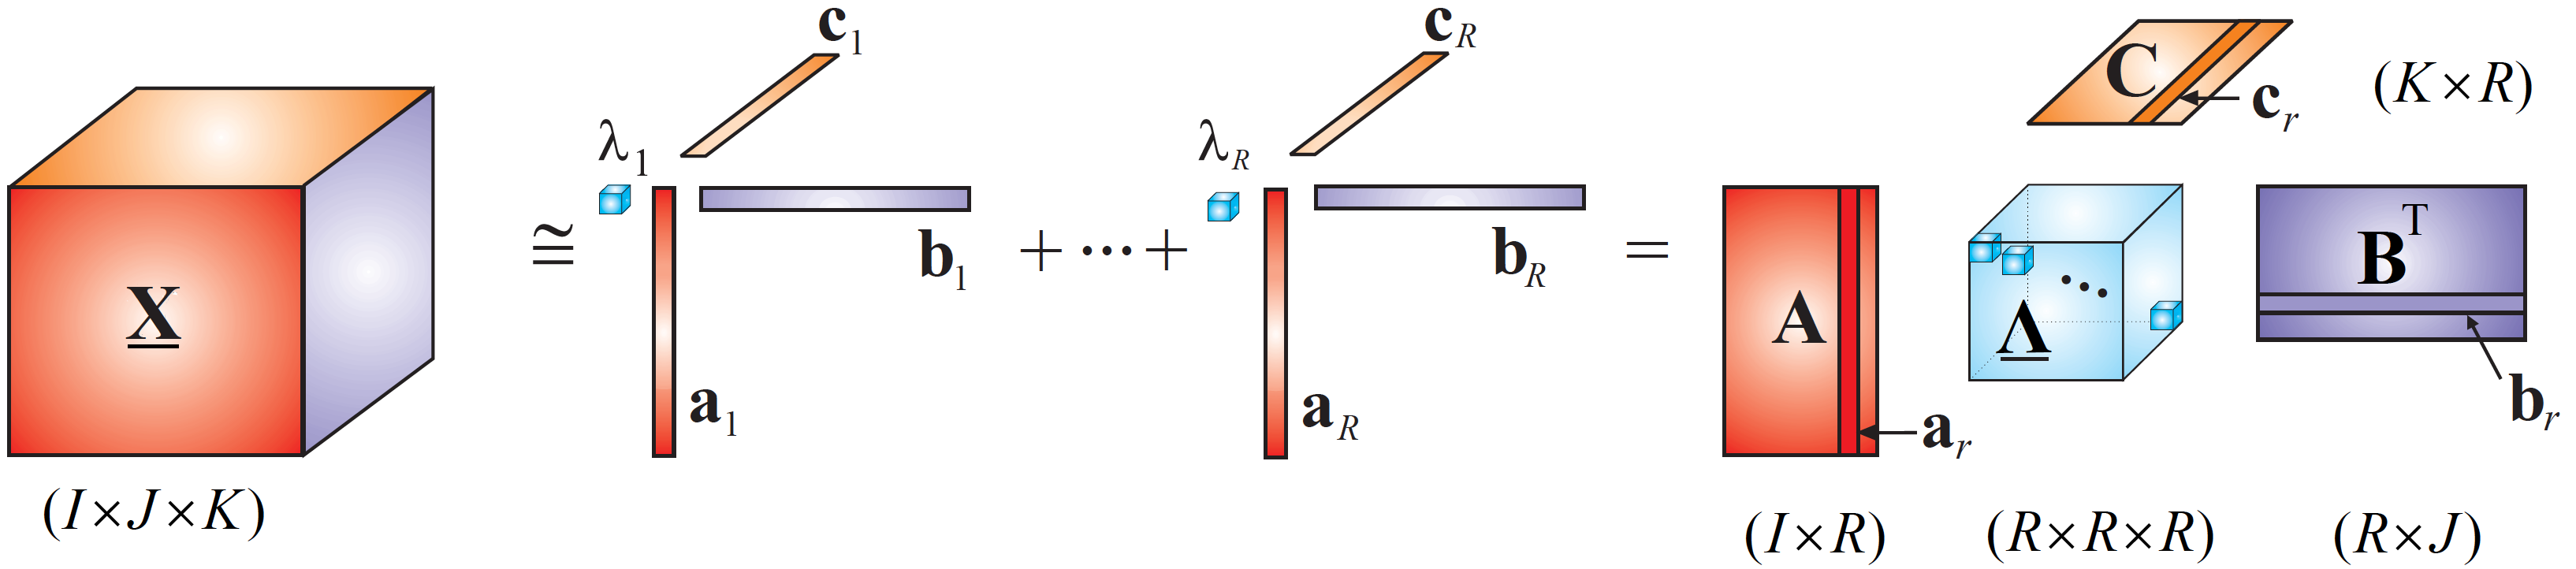
\includegraphics[width=0.6\textwidth]{figures/cpd_decomp}
\caption{CPD decomposition}
\label{fig:Lab1:2}
\end{figure}

Consider a 3-rd order tensor $\mathbf{\underline{X}} \in \mathbb{R}^{I \times J \times K}$. We define its CPD Decomposition as 

\begin{equation}
\begin{aligned}
\mathbf{\underline{X}} & \simeq \sum_{r=1}^{R} \lambda_r \mathbf{a}_r \circ \mathbf{b}_r \circ \mathbf{c}_r\\
& = \mathbf{\underline{\Lambda}} \times_1 \mathbf{A} \times_2 \mathbf{B} \times_3 \mathbf{C}\\
& = \Big[    \mathbf{\underline{\Lambda}} ;  \mathbf{A},  \mathbf{B}, \mathbf{C}      \Big]
\end{aligned}
\end{equation}

where $\mathbf{\underline{\Lambda}}$ is a 3-rd order core tensor having $\lambda_r$ as entries at positions $\mathbf{\underline{\Lambda}}[i, j, k]$ where $\mathbf{\underline{\Lambda}}[i, j, k]$ and zeros elsewhere; $\mathbf{A}, \mathbf{B}, \mathbf{C}$ are factor matrices obtained as the concatenation of the corresponding factor vectors, i.e $\mathbf{A} = \Big[    \mathbf{a}_1 \mathbf{a}_2  \cdots \mathbf{a}_R   \Big]$.

\subsection{Experiments}

\textbf{NB:} Jupyter Notebook with the code can be found at \url{https://github.com/evgeniishch/mm_forecasting}.

As an experiment both HOSVD and CPD decompositions are applied to 3-dimensional tensors. 

\subsection{RGB image}

RGB image is formally a 3-dimensional tensor, however not completely honest as its RBG features are unordered and can be viewed as categorical. Yet it is good to start with.

A $100 \times 100 \times 3$ RGB image tensor is decomposed via HOSVD and CPD algorithms:

\begin{figure}[h!]
\centering
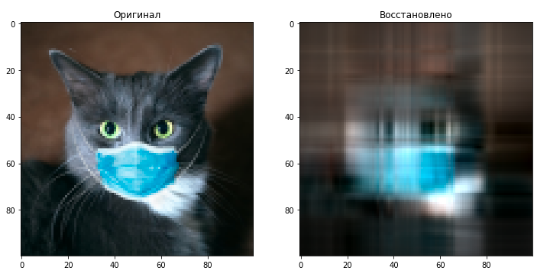
\includegraphics[width=0.6\textwidth]{figures/tucker_img}
\caption{Comparison of original image and image reconstructed from HOSVD decomposition with rank 5}
\label{fig:Lab1:3}
\end{figure}

\begin{figure}[h!]
\centering
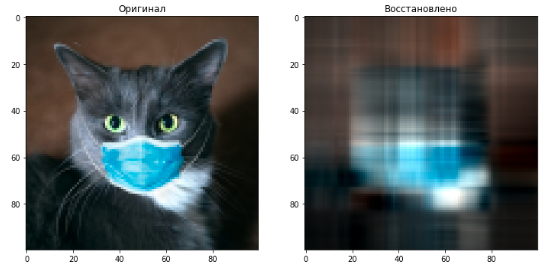
\includegraphics[width=0.6\textwidth]{figures/cpd_img}
\caption{Comparison of original image and image reconstructed from CPD decomposition with rank 5}
\label{fig:Lab1:4}
\end{figure}

For each decomposed tensor a residual tensor is computed and relative error of approximation is calculated w.r.t. decomposition rank:


\begin{figure}[h!]
\centering
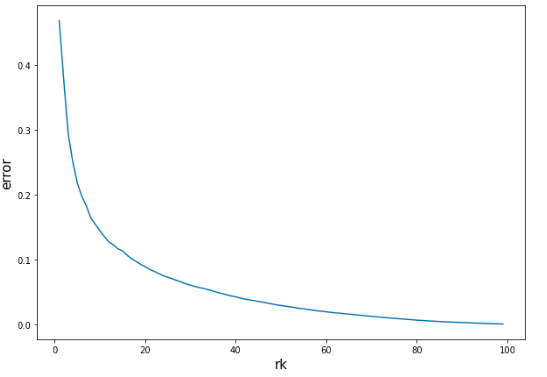
\includegraphics[width=0.6\textwidth]{figures/HOSVD_err}
\caption{Relative error of HOSVD decomposition w.r.t. decomposition rank}
\label{fig:Lab1:5}
\end{figure}

\begin{figure}[h!]
\centering
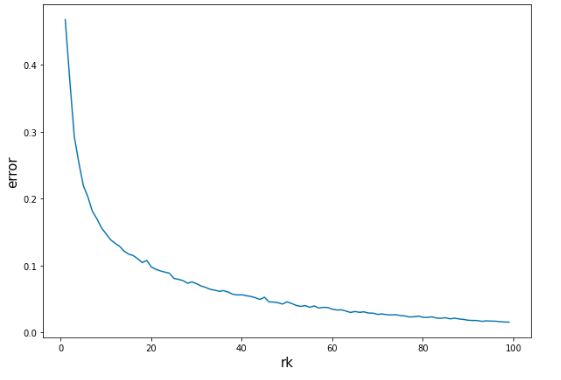
\includegraphics[width=0.6\textwidth]{figures/CPD_err}
\caption{Relative error of CPD decomposition w.r.t. decomposition rank}
\label{fig:Lab1:6}
\end{figure}

For entertainment purposes, a picture of a dog and a picture of a cake are decomposed with CPD algorithm. We offer the reader to distinguish between them at decomposition rank $2$:

\begin{figure}[h!]
\centering
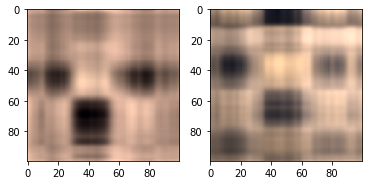
\includegraphics[width=0.6\textwidth]{figures/cakedog}
\caption{Try to distinguish Chihua-hua and a cake}
\label{fig:Lab1:7}
\end{figure}

\subsubsection{Animation film}

Earlier, we considered images, which, although they are three-dimensional tensors, are of less interest for research, since the order is not defined on the features for one of the dimensions (RGB). Next, a short gray scale animation film is used as data for decomposition.

A $500 \times 333 \times 69$ frame sequence tensor is decomposed via CPD algorithm. A residual tensor is computed and relative error of approximation is calculated w.r.t. decomposition rank:

\begin{figure}[h!]
\centering
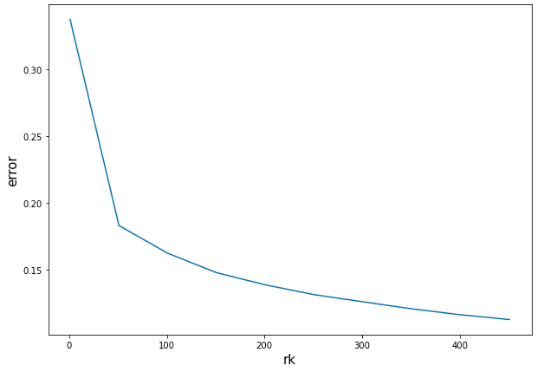
\includegraphics[width=0.6\textwidth]{figures/mickey_err}
\caption{Relative error of CPD decomposition w.r.t. decomposition rank}
\label{fig:Lab1:8}
\end{figure}

From visual observation a higher reconstruction quality is noticed for regions with high pixel contrast. 


\end{document}